\section{2D Burgers Equation}

\begin{secframe}
\small
\textcolor{red_unipd}{\Large Section Overview}

\begin{alertblock}{Goal}
    Compare a physical simulator and a Neural Field Turing Machine (NFTM) for solving the 2D Burgers equation.

\end{alertblock}

\begin{block}{Approach}
Build a numerical solver, then train and evaluate NFTM on the same problem.
\end{block}
\end{secframe}

% ===== Slide 1 =====
\begin{secframe}
\small
\textcolor{red_unipd}{\Large Governing Equations}

\vspace{0.6em}

\begin{alertblock}{Equation}
\[
\begin{cases}
  u_t + u u_x + v u_y = \nu (u_{xx} + u_{yy}), \\
  v_t + u v_x + v v_y = \nu (v_{xx} + v_{yy})
\end{cases}
\]
\end{alertblock}

\vfill

\begin{block}{Hypotheses}
\(\nabla p=\mathbf{0}\). \quad
1D reduction: \(\mathbf{u}=(u(x,t),0)\). \quad
Self-advection: \(u\,\partial_x u\).
\end{block}

\vspace{0.5em}

\begin{block}{Einstein notation}
$u_t = \frac{\partial u}{\partial t}$, $u_x = \frac{\partial u}{\partial x}$, $u_{xx} = \frac{\partial^2 u}{\partial x^2}$, etc.
\end{block}

\end{secframe}

% ===== Advection Frame =====
\begin{secframe}
\small
\textcolor{red_unipd}{\Large Advection}

\vspace{0.6em}

\begin{block}{Advection Terms}
\begin{itemize}
    \item \textbf{$u u_x$, $v v_y$, $u v_x$, $v u_y$}: Nonlinear advection terms.
    \item Represent transport of velocity due to the flow itself.
\end{itemize}
\end{block}

\begin{figure}[h]
    \centering
    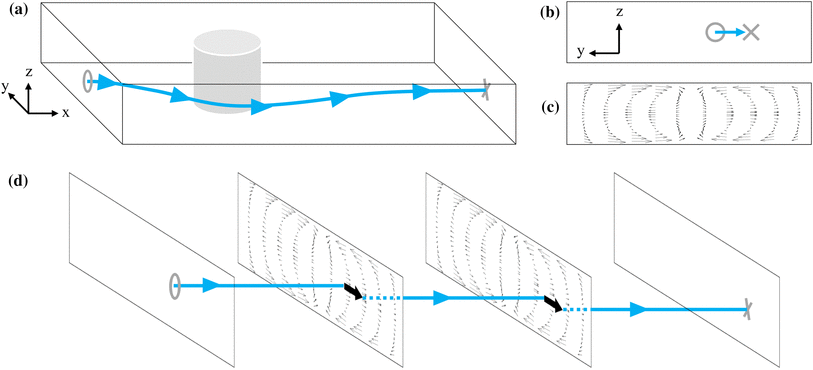
\includegraphics[width=0.7\linewidth]{images/theory/advection.png}
\end{figure}

\end{frame}

% ===== Diffusion Frame =====
\begin{frame}{2D Burgers Equation}
\small
\textcolor{red_unipd}{\Large Diffusion}

\vspace{0.6em}

\begin{block}{Diffusion Terms}
\begin{itemize}
    \item \textbf{$\nu (u_{xx} + u_{yy})$, $\nu (v_{xx} + v_{yy})$}: Diffusion terms.
    \item Model the spreading and smoothing of velocity due to viscosity $\nu$.
\end{itemize}
\end{block}

\begin{figure}[h]
    \centering
    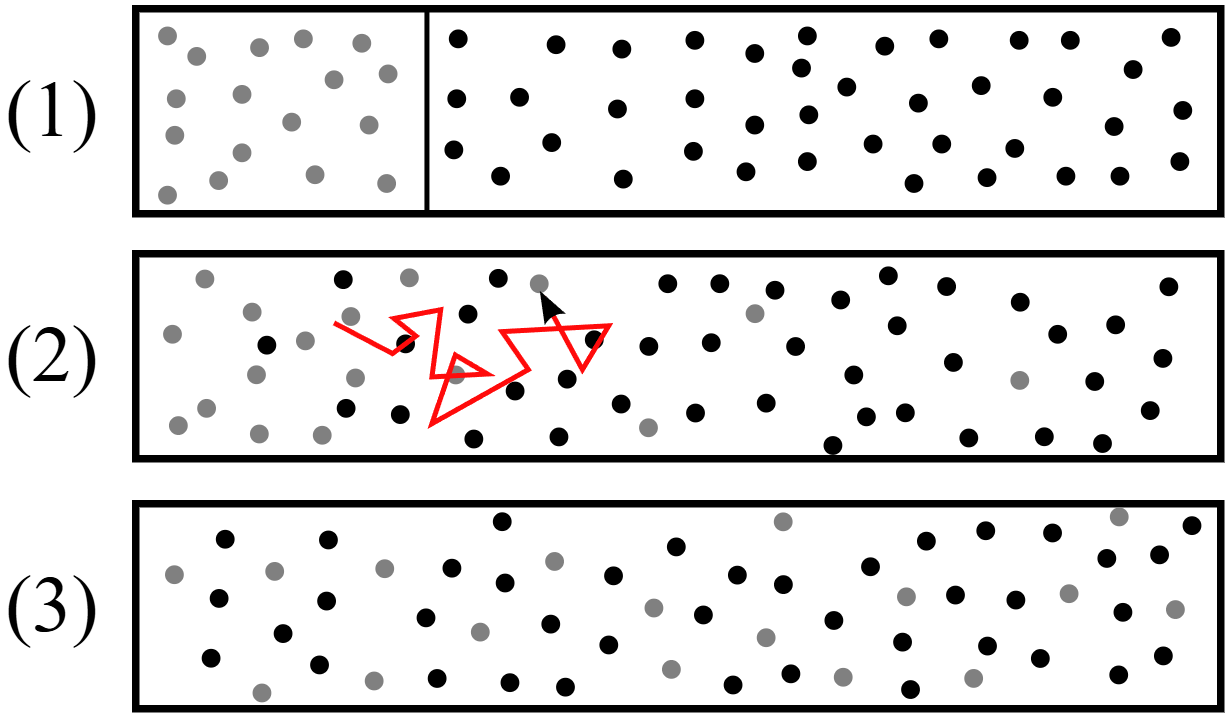
\includegraphics[width=0.7\linewidth]{images/theory/diffusion.png}
\end{figure}


\end{secframe}

% ===== Balance Frame =====
\begin{secframe}
\small
\textcolor{red_unipd}{\Large Pressure gradient}

\vspace{0.6em}

\begin{alertblock}{Pressure Gradient Terms}
  The huge Hypotheses here is \(\nabla p=\mathbf{0}\), so there is no effect of the pressure in the equation. \\
  \( \Rightarrow \) Only the initial velocity has an influence on the evolution of the system
\end{alertblock}

\begin{example}
  Consider a scenario where the initial velocity is constant across the domain on airfoil shape. \\
  Since \(\nabla p=\mathbf{0}\), the pressure gradient does not influence the flow. \\
  The flow will not change over time, remaining constant as per the initial condition.
\end{example}



\end{secframe}

% ===== Slide 2 =====
\begin{secframe}
\small
\textcolor{red_unipd}{\Large Numerical Simulation}

\vspace{0.6em}

\begin{block}{Description}
\begin{itemize}
  \item Implements the PDE directly using finite difference methods.
  \item Discretizes space and time; updates velocity fields step by step.
  \item Parameters: grid size, time step, viscosity, initial/boundary conditions.
\end{itemize}
\end{block}

\begin{alertblock}{Finite Difference Schemes}
\begin{itemize}
  \item Forward difference (time): $u_t \approx \frac{u_{i,j}^{n+1} - u_{i,j}^n}{\Delta t}$
  \item Central difference (space): $u_x \approx \frac{u_{i+1,j}^n - u_{i-1,j}^n}{2\Delta x}$
  \item Central difference (second derivative): $u_{xx} \approx \frac{u_{i+1,j}^n - 2u_{i,j}^n + u_{i-1,j}^n}{\Delta x^2}$
\end{itemize}
\end{alertblock}

\end{secframe}

% ===== Slide 3 =====
\begin{secframe}
\small
\textcolor{red_unipd}{\Large Neural Field Turing Machine}

\vspace{0.6em}

\begin{alertblock}{Objective}
\begin{itemize}
  \item Learns to update field values using neural controllers and local memory patches.
  \item Trained on data from the physical simulator or existing datasets.
  \item Can generalize to new initial conditions or parameters.
\end{itemize}
\end{alertblock}

\begin{block}{Datasets}
\begin{itemize}
  \item Use existing benchmark datasets for PDEs (if available).
  \item Generate custom datasets using our physical simulator (varied initial/boundary conditions, parameters).
\end{itemize}
\end{block}
\end{secframe}


% ===== Slide 5 =====
\begin{secframe}
\small
\textcolor{red_unipd}{\Large Summary \& Next Steps}

\vspace{0.6em}

\begin{block}{Next Steps}
\begin{itemize}
  \item Build and validate the physical simulator.
  \item Train NFTM on generated and existing datasets.
  \item Compare performance, accuracy, and generalization.
\end{itemize}
\end{block}
\end{secframe}